
\section{Supermassive Black Hole Growth}
\label{sec:smbh_growth}

Supermassive black holes grow by two primary mechanisms, binary mergers and gas accretion.  Through a combination of these, black holes can grow to as large as $\sim 10^{9}$--$10^{10}$~M$_{\odot}$ by $z = 0$.



%%%%%%%%%%%%%%%%%%%%%%%%%%%%%%%%%%%%%%%%%%%%%%%%%%%%
\subsection{Binary Mergers}

When two galaxies merge, the supermassive black holes at their hearts begin a process that will eventually lead to their coalescence.  There are generally thought to be three stages to this journey.  First, the black holes sink towards the center of the merged galaxy through mass segregation and dynamical friction until they form a bound orbit with each other.  Then, the black holes tighten their orbit through three-body scattering of nearby stars.  Finally, as the black holes become close enough together for general relativistic effects to come into play, gravitational waves are emitted and radiate away the remaining orbital energy until the binary coalesces.


%---------------------------------------------------
\subsubsection{Dynamical Friction and Inspiral}

During the majority of the inspiral process, the black holes do not ``feel'' each other's gravitational pull.  Instead, interactions with the galaxy itself push the holes together.

As it travels through a galaxy, a black hole---or any massive body---is slowed by the surrounding field of matter.  Gravitational attraction pulls surrounding matter toward the black hole.  However, as the black hole is moving with respect to the local medium, the attracted particles will tend to fall behind the black hole.  This creates a wake of overdensity that gravitationally attracts the black hole from behind and slows its velocity.  \citet{chandrasekhar_1943} develops this notion of dynamical friction for the motion of a star through a sea of other stars.  If the distribution of velocities of the surrounding particles is Maxwellian, the acceleration on the black hole can be written as
\begin{equation} \label{eq:dynamical_friction}
  \frac{d\mathbf{v}_{M}}{dt} = - \frac{4 \pi G^{2} M \rho \ln \Lambda}{v_{M}^{3}} \left[ \textrm{erf}(X) - \frac{2X}{\sqrt{\pi}} e^{-X^{2}} \right] \mathbf{v}_{M},
\end{equation}
where $\mathbf{v}_{M}$ is the velocity of the black hole, $M$ is it's mass, $\rho$ is the density of surrounding matter, $\textrm{erf}$ is the error function, $\ln \Lambda$ is the Coulomb logarithm, and $X \equiv v_{M} / (\sqrt{2} \sigma)$ where $\sigma$ is the velocity dispersion of the surrounding medium \citep{binney_tremaine_1988}.  As the black hole is slowed by dynamical friction, it loses angular momentum and sinks towards the center of the galaxy's potential well.


%---------------------------------------------------
\subsubsection{The Final Parsec Problem}

Dynamical friction and mass segregation can only take us so far.  Once the black holes are close enough together, they form a bound binary orbit.  This generally occurs for separations of around a few to tens of parsecs.  This presents a problem, however, since the orbit needs to shrink to around $10^{-2}$--$10^{-3}$ pc in order for gravitational wave emission to remove energy from the orbit in a significant amount.  The orbit can be tightened with three-body scattering of stars that wander through the orbit of the binary, however, in the spherical galaxies where mergers often take place, there is a depletion of stars with orbits that intersect the binary.  \citet{khan_2011}, however, show that the non-spherical, triaxial potential typical of post-merger galaxy remnants can efficiently funnel stars through the orbit of the black hole binary with sufficient intensity to tighten the binary orbit to the gravitational wave regime.


%---------------------------------------------------
\subsubsection{Gravitational Waves and Recoil Kicks}

Once the black hole binary separation reaches the point where strong field general relativistic effects come into play, we no longer require external influences to nudge the black holes together.  In the final plunge toward coalescence, the black hole binary sheds energy through emission of gravitational radiation.  As energy is radiated away, the binary tightens its orbit until the two black holes merge into one.  Following this coalescence, the resultant black hole undergoes a ``ringdown'' phase, in which the distorted space time settles back down into a black hole that can again be simply described by mass, charge, and spin.

The emission of gravitational waves has two interesting consequences.  First, the radiation from two merging supermassive black holes is extremely loud, and can potentially provide an observational signature of the process for gravitational wave observatories.  Second, the gravitational waves carry linear momentum, leading to a recoil ``kick'' imparted to the black hole merger remnant.

Recent advances in numerical relativity simulations have provided a much deeper insight into the black hole binary merger process than has been previously available.  Waveforms produced from these simulations (Figure~\ref{fig:waveform}) can be used to predict what gravitational wave observatories such as LIGO and LISA would expect to observe for signals originating from merging supermassive black hole binaries.  Having these waveforms as templates for comparison to data can greatly increase the signal to noise ratio for these detectors, potentially allowing the gravitational wave events to be seen among the sea of noise.  These waveforms produced from simulations of the last few orbits of inspiral through the merger and ringdown can be combined with waveforms suggested from post-Newtonian approximations for the longer duration inspiral to provide a complete extended signal to match against.

\begin{figure}[t]
\centering
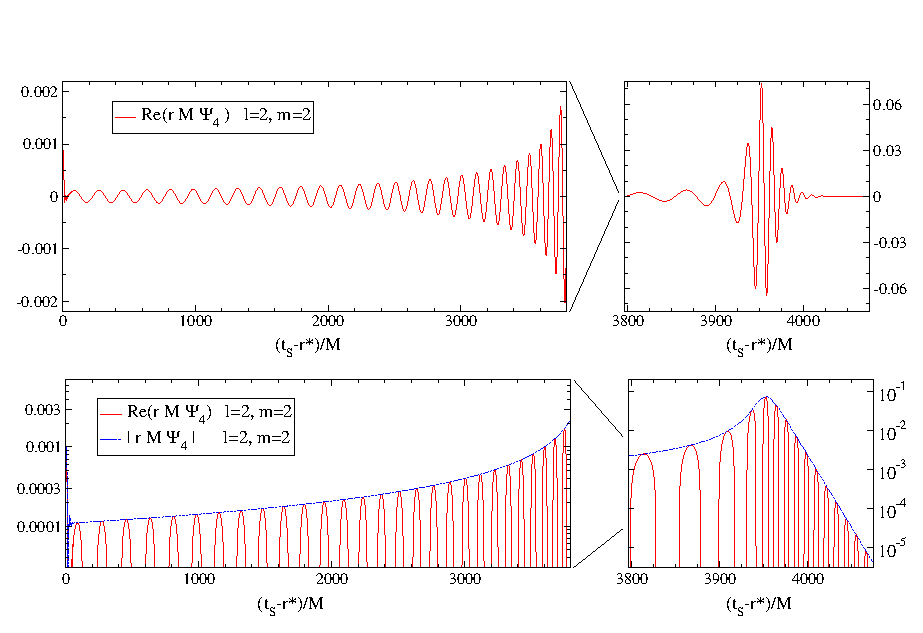
\includegraphics[width=\linewidth]{scheel_2009_waveform.eps}
\caption[Gravitational waveform for a black hole binary merger]{\footnotesize Gravitational waveform for an equal-mass, non-spinning black hole binary merger. This is the final waveform, extrapolated to infinity, from the numerical relativity simulation of \citet{scheel_2009}.  The waveform is shown on the top panel with a linear y-axis and on the bottom panel with a logarithmic y-axis.  The left panels are the earlier stages of inspiral, and the right panels show the merger and ringdown stages.}
\label{fig:waveform}
\end{figure}

For asymmetric mergers, gravitational radiation is emitted anisotropically.  This causes a recoil kick, in which the gravitational waves impart a net velocity to the final black hole with respect to the original center of mass.  The magnitude and direction of this kick are dependent on the mass ratio of the binary and the spins of the two black holes---in all, a 7-dimensional parameter space.  This large parameter space has been largely explored with numerical relativistic simulations, and analytic equations can be fit to the data to predict the recoil from a given merger configuration.  \citet{holley-bockelmann_2008}, give these equations as
\begin{equation} \label{eq:v_kick}
  \mathbf{v}_{kick} = \left(1+e\right)\left[\mathbf{\hat{x}}\left(v_{m} + v_{\perp} \cos\xi\right) + \mathbf{\hat{y}}v_{\perp}\sin\xi + \mathbf{\hat{z}}v_{\parallel}\right],
\end{equation}
where 
\begin{equation} \label{eq:v_m}
  v_{m} = A \frac{q^{2}(1-q)}{(1+q)^{5}} \left[1 + B \frac{q}{(1+q)^{2}}\right],
\end{equation}
\begin{equation} \label{eq:v_perp}
  v_{\perp} = H \frac{q^{2}}{\left(1+q\right)^{5}} \left(\alpha_{2}^{\parallel} - q\alpha_{1}^{\parallel}\right),
\end{equation}
\begin{equation} \label{eq:v_parallel}
  v_{\parallel} = K \cos\left(\Theta - \Theta_{0}\right) \frac{q^{2}}{\left(1+q\right)^{5}} \left(\alpha_{2}^{\perp} - q\alpha_{1}^{\perp}\right).
\end{equation}
Here, the fitting constants are $A = 1.2 \times 10^{4}$ km~s$^{-1}$, $B = -0.93$, $H = (7.3 \pm 0.3) \times 10^{3}$ km~s$^{-1}$, and  $K = (6.0 \pm 0.1) \times 10^{4}$ km s$^{-1}$.  The $\hat{z}$ unit vector is in the direction of the orbital angular momentum, and $\perp$ and $\parallel$ refer to components perpendicular and parallel to $\hat{z}$, respectively.  The fitting parameters are the eccentricity $e$, the mass ratio $q \equiv M_{2}/M_{1}$, and the reduced spin parameters $\alpha_{i} \equiv S_{i}/M_{i}^{2}$ where $S$ is the spin angular momentum.  The orientation of the merger is given by the angles $\Theta$, $\Theta_{0}$, and $\xi$ \citep{holley-bockelmann_2008}.

Slices through this parameter space are shown in Figure~\ref{fig:recoil_kicks}.  For certain configurations of the merger, the recoil velocity can be very high.  Very asymmetric mergers can produce recoils as high as $\sim 4000$ km s$^{-1}$.  These large recoils can be enough for the black hole to escape the potential well of its host galaxy and be ejected.  Even less extreme recoil kicks can affect the evolution of black holes, as the kicked black hole can oscillate about its host's center, potentially changing its local gas environment and accretion rate.

\begin{figure}[t]
\centering
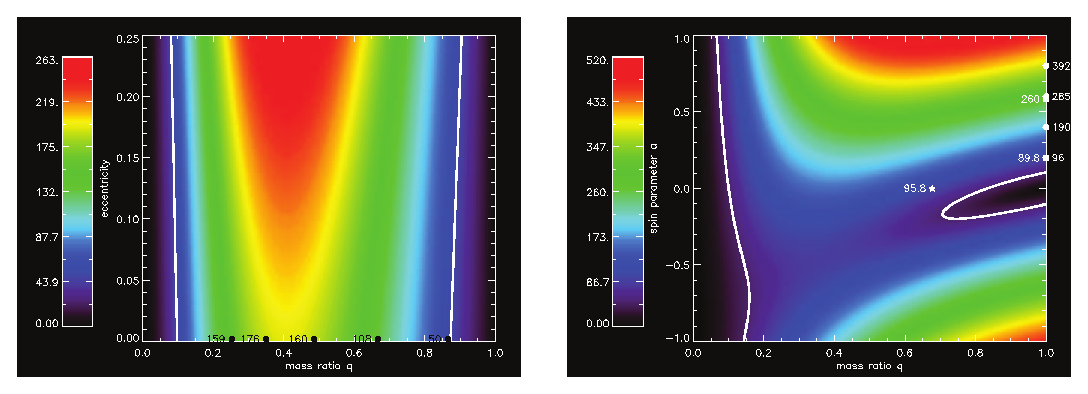
\includegraphics[width=\linewidth]{holley-bockelmann_2008_recoil_kicks.eps}
\caption[Gravitaional wave recoil velocity from black hole mergers]{\footnotesize \textit{Left:} Gravitaional wave recoil velocity from a merger of nonspinning black holes as a function of eccentricity and mass ratio.  Data from numerical relativity simulations \citep{gonzalez_2007} are overlaid along the zero eccentricity line.  The overlaid white contours are the escape velocity of a typical globular cluster, 50 km s$^{-1}$.  \textit{Right:} Gravitational wave recoil kick velocity as a function of spin parameter and mass ratio for a merger of spinning black holes on a circular orbit with spins perpendicular to the orbital plane of the binary and anti-aligned with each other.  Again, the 50 km s$^{-1}$ escape velocity of a globular cluster is overlaid as white contours.  Results from numerical relativity simulations are over-plotted:  squares for \citet{koppitz_2007}, cirlces for \citet{herrmann_2007}, and star for \citet{brugmann_2004}.  \citep{holley-bockelmann_2008}}
\label{fig:recoil_kicks}
\end{figure}



%%%%%%%%%%%%%%%%%%%%%%%%%%%%%%%%%%%%%%%%%%%%%%%%%%%%
\subsection{Accretion}

Although mergers play an important role in the evolution of supermassive black holes, gas accretion can often dominate in terms of mass growth.  Gas can fall into a black hole in a number of ways.  Here, we will discuss accretion onto a moving black hole, spherical accretion onto a stationary black hole, and disk accretion onto a stationary black hole.


%---------------------------------------------------
\subsubsection{Bondi-Hoyle-Lyttleton Accretion}

Let us first consider a massive object, in this case our black hole, moving through a uniform density gas medium.  Just as in the case of dynamical friction, particles close enough to the black hole will feel a gravitational attraction, causing them to move toward the black hole.  As they move closer, the black hole is also moving through the medium, causing the gas particles to focus behind the black hole.  As the particle stream reaches the wake directly behind the black hole, it collides with opposing streams, causing the angular momentum to go to zero.  If these particles are bound, they will proceed to fall onto the black hole.  \citet{hoyle_1939} derive an impact parameter for which particles will be accreted,
\begin{equation} \label{eq:sigma}
  \sigma < \sigma_{HL} = \frac{2GM}{v_{\infty}^{2}},
\end{equation}
and a mass accretion from the wake column at a rate of
\begin{equation} \label{eq:Mdot_HL}
  \dot{M}_{HL} = \pi \sigma_{HL}^{2} v_{\infty} \rho_{\infty} = \frac{4 \pi G^{2} M^{2} \rho_{\infty}}{v_{\infty}^{3}},
\end{equation}
where $v_{\infty}$ and $\rho_{\infty}$ are the velocity and density far away from the black hole, respectively.  Expanding upon this analysis, \citet{bondi_1944} suggest that the accretion rate should rather be
\begin{equation} \label{eq:Mdot_BH_1}
  \dot{M}_{BH} = \frac{2 \alpha \pi G^{2} M^{2} \rho_{\infty}}{v_{\infty}^{3}},
\end{equation}
where $\alpha$ is a constant between $1$ and $2$, with a typical value of around $1.25$.

For an accretor at rest in an isotropic gas medium, one would expect accretion to be a spherical process.  \citet{bondi_1952} considers this configuration, and finds the accretion rate for this ``temperature-limited'' case to be
\begin{equation} \label{eq:Mdot_Bondi}
  \dot{M}_{Bondi} = \frac{2 \pi G^{2} M^{2} \rho_{\infty}}{c_{s,\infty}^{3}},
\end{equation}
where $c_{s,\infty}$ is the speed of sound far away from the black hole.

Extrapolating between this result and the ``velocity-limited'' case of Equation~\ref{eq:Mdot_BH_1} suggests \citep{bondi_1952}
\begin{equation} \label{eq:Mdot_BH_2}
  \dot{M}_{BH} = \frac{2 \pi G^{2} M^{2} \rho_{\infty}}{\left(c_{s,\infty}^{2} + v_{\infty}^{2}\right)^{3/2}}
\end{equation}
as an order of magnitude estimate of the more general case of accretion.  Numerical simulations \citep{shima_1985} suggest an additional factor of $2$ is needed for better agreement with simulation results, giving us a generally applicable from for the accretion rate,
\begin{equation} \label{eq:Mdot_BH_3}
  \dot{M}_{BH} = \frac{4 \pi G^{2} M^{2} \rho_{\infty}}{\left(c_{s,\infty}^{2} + v_{\infty}^{2}\right)^{3/2}}.
\end{equation}


%---------------------------------------------------
\subsubsection{Disk Accretion and Active Galactic Nuclei}

Active galactic nuclei play a fundamental role in the evolution of both supermassive black holes and their host galaxies.  As gas falls in to a black hole in the center of a galaxy, its angular momentum forces it into an accretion disk.  As matter moves towards the SMBH, it transfers its gravitational potential energy to thermal energy.  For accretion disks around supermassive black holes, this can cause the disk to emit large amounts of electromagnetic radiation \citep{lin_1996}.

This emitted radiation is important in a number of ways.  Most critical to the SMBH itself is the radiation pressure exerted on infalling matter.  This radiation pressure sets an upper limit on the rate of accretion, as there is a point where the force from emitted radiation balances the force of gravity for infalling gas \citep{rybicki_lightman_1979}.  This limit, known as the Eddington limit, is given by
\begin{equation} \label{eq:L_Edd}
  L_{Edd} = 4 \pi G M c m_{H} / \sigma_{T} = 1.25 \times 10^{38} \textrm{erg s}^{-1} (M / M_{\odot}),
\end{equation}
where $c$ is the speed of light, $m_{H}$ is the mass of hydrogen, and $\sigma_{T}$ is the Thompson cross section.

The radiation given off by the accretion disk affects galactic properties as well.  Powerful AGN can strip away gas from the center of the galaxy, halting star formation.  This can quickly change a galaxy from a blue, gaseous, star forming galaxy into one that is red, dry, and dead.



